%beamer

% This video for Turing:
% https://www.youtube.com/watch?v=VxvY4rI15sM

% Comment/uncomment this line to toggle handout mode
\newcommand{\handout}{}

%% Beamer-Klasse im korrekten Modus
\ifdefined \handout
\documentclass[handout]{beamer} % Handout mode
\else
\documentclass{beamer}
\fi

%% UTF-8-Encoding
\usepackage[utf8]{inputenc}

\input{../framework/gbi-macros}
\usepackage[blue]{../framework/thwregex}
\usepackage{environ}
\usepackage{bm}
\usepackage{calc}
\usepackage{varwidth}
\usepackage{wasysym}
\usepackage{mathtools}


% Das ist der KIT-Stil
%\usepackage{../TutTexbib/beamerthemekit}
\usepackage[deutsch,titlepage0]{../framework/KIT/beamerthemeKITmod}
\TitleImage[width=\titleimagewd]{../figures/titlepage.jpg}
%\usetheme[deutsch,titlepage0]{KIT}

% Include PDFs
\usepackage{pdfpages}

% Libertine font (Original GBI font)
\usepackage{libertine}
%\renewcommand*\familydefault{\sfdefault}  %% Only if the base font of the document is to be sans serif

% Nicer math symbols
\usepackage{eulervm}
%\usepackage{mathpazo}
\renewcommand\ttdefault{cmtt} % Computer Modern typewriter font, see lecture slides.

\usepackage{csquotes}

%%%%%%

%% Schönere Schriften
\usepackage[TS1,T1]{fontenc}

%% Bibliothek für Graphiken
\usepackage{graphicx}

%% der wird sowieso in jeder Datei gesetzt
\graphicspath{{../figures/}}

%% Anzeigetiefe für Inhaltsverzeichnis: 1 Stufe
\setcounter{tocdepth}{1}

%% Hyperlinks
\usepackage{hyperref}
% I don't know why, but this works and only includes sections and NOT subsections in the pdf-bookmarks.
\hypersetup{bookmarksdepth=subsection} 

%\usepackage{lmodern}
\usepackage{colortbl}
\usepackage[absolute,overlay]{textpos}
\usepackage{listings}
\usepackage{forloop}
%\usepackage{algorithmic} % PseudoCode package 

\usepackage{tikz}
\usetikzlibrary{matrix}
\usetikzlibrary{arrows.meta}
\usetikzlibrary{automata}
\usetikzlibrary{tikzmark}
\usetikzlibrary{positioning}

% Why has no-one come up with this yet? I mean, seriously. -.-
\tikzstyle{loop below right} = [loop, out=-60,in=-30, looseness=7]
\tikzstyle{loop below left} = [loop, out=-150,in=-120, looseness=7]
\tikzstyle{loop above right} = [loop, out=60,in=30, looseness=7]
\tikzstyle{loop above left} = [loop, out=150,in=120, looseness=7]
\tikzstyle{loop right below} = [loop below right]
\tikzstyle{loop left below} = [loop below left]
\tikzstyle{loop right above} = [loop above right]
\tikzstyle{loop left above} = [loop above left]

% Needed for gbi-macros
\usepackage{xspace}

%%%%%%

%% Verbatim
\usepackage{moreverb}

%%%%%%%%%%%%%%%%%%%%%%%%%%%%%%%%%%%% Copy end

%% Tabellen
\usepackage{array}
\usepackage{multicol}
\usepackage{hhline}

%% Bibliotheken für viele mathematische Symbole
\usepackage{amsmath, amsfonts, amssymb}

%% Deutsche Silbentrennung und Beschriftungen
\usepackage[ngerman]{babel}

\usepackage{kbordermatrix}

% kbordermatrix settings
\renewcommand{\kbldelim}{(} % Left delimiter
\renewcommand{\kbrdelim}{)} % Right delimiter

\input{../config.tex}



% define custom \handout command flag if handout mode is toggled  #DirtyAsHellButWell...
\only<beamer:0>{\def\handout{}} %beamer:0 == handout mode

\newcommand{\R}{\mathbb{R}}
\newcommand{\N}{\mathbb{N}}
\newcommand{\Z}{\mathbb{Z}}
\newcommand{\Q}{\mathbb{Q}}
\newcommand{\BB}{\mathbb{B}}
\newcommand{\C}{\mathbb{C}}
\newcommand{\K}{\mathbb{K}}
\newcommand{\G}{\mathbb{G}}
\newcommand{\nullel}{\mathcal{O}}
\newcommand{\einsel}{\mathds{1}}
\newcommand{\Pot}{\mathcal{P}}
\renewcommand{\O}{\text{O}}

\def\word#1{\hbox{\textcolor{blue}{\texttt{#1}}}}
\let\literal\word
\def\mword#1{\hbox{\textcolor{blue}{$\mathtt{#1}$}}}  % math word
\def\sp{\scalebox{1}[.5]{\textvisiblespace}}
\def\wordsp{\word{\sp}}

%\newcommand{\literal}[1]{\textcolor{blue}{\texttt{#1}}}
\newcommand{\realTilde}{\textasciitilde \ }
\newcommand{\setsize}[1]{\ensuremath{\left\lvert #1 \right\rvert}}
\newcommand{\size}[1]{\setsize{#1}}  % Shame on you, TeXStudio...
\newcommand{\set}[1]{\left\{#1\right\}}
\newcommand{\tuple}[1]{\left(#1\right)}
\newcommand{\normalvar}[1]{\text{$#1$}}

% Modified by DJ
\let\oldemptyset\emptyset
\let\emptyset\varnothing % proper emptyset

\newcommand{\boder}{\ensuremath{\mathbin{\textcolor{blue}{\vee}}}\xspace}
\newcommand{\bund}{\ensuremath{\mathbin{\textcolor{blue}{\wedge}}}\xspace}
\newcommand{\bimp}{\ensuremath{\mathrel{\textcolor{blue}{\to}}}\xspace}
\newcommand{\bgdw}{\ensuremath{\mathrel{\textcolor{blue}{\leftrightarrow}}}\xspace}
\newcommand{\bnot}{\ensuremath{\textcolor{blue}{\neg}}\xspace}
\newcommand{\bone}{\ensuremath{\textcolor{blue}{1}}\text{}}
\newcommand{\bzero}{\ensuremath{\textcolor{blue}{0}}\text{}}
\newcommand{\bleftBr}{\ensuremath{\textcolor{blue}{\texttt{(}}}\text{}}
\newcommand{\brightBr}{\ensuremath{\textcolor{blue}{\texttt{)}}}\text{}}

% Fix of \b... commands:

\renewcommand{\boder}{\alor}
\renewcommand{\bund}{\aland}
\renewcommand{\bimp}{\alimpl}
\renewcommand{\bgdw}{\aleqv}
\renewcommand{\bnot}{\alnot}
\renewcommand{\bleftBr}{\alka}
\renewcommand{\brightBr}{\alkz}
\newcommand{\alA}{\word A}
\newcommand{\alB}{\word B}
\newcommand{\alC}{\word C}

\newcommand{\plB}{\plfoo{B}}
\newcommand{\plE}{\plfoo{E}}

\newcommand{\summe}[2]{\sum\limits_{#1}^{#2}}
\newcommand{\limes}[1]{\lim\limits_{#1}}

%\newcommand{\numpp}{\advance \value{weeknum} by -2 \theweeknum \advance \value{weeknum} by 2}
%\newcommand{\nump}{\advance \value{weeknum} by -1 \theweeknum \advance \value{weeknum} by 1}

\newcommand{\mycomment}[1]{}
\newcommand{\Comment}[1]{}

%% DISCLAIMER START 
% It is INSANELY IMPORTANT NOT TO DO THIS OUTSIDE BEAMER CLASS! IN ARTCILE DOCUMENTS, THIS IS VERY LIKELY TO BUG AROUND!
\makeatletter%
\@ifclassloaded{beamer}%
{
	% TODO 
	% no time... later.   (= never -.-)
	% redefine section to ignore multiple \section calls with the same title
}%
{
	\errmessage{ERROR: section command redefinition outside of beamer class document! Please contact the author of this code or read the F-ing disclaimer.}
}%
\makeatother%
%% DISCLAIMER END

\newcounter{abc}
\newenvironment{alist}{
  \begin{list}{(\alph{abc})}{
      \usecounter{abc}\setlength{\leftmargin}{8mm}\setlength{\labelsep}{2mm}
    }
}{\end{list}}


\newcommand{\stdarraystretch}{1.20}
\renewcommand{\arraystretch}{\stdarraystretch}  % for proper row spacing in tables

\newcommand{\morescalingdelimiters}{   % for proper \left( \right) typography
	\delimitershortfall=-1pt  
	\delimiterfactor=1
}

\newcommand{\centered}[1]{\vspace{-\baselineskip}\begin{center}#1\end{center}\vspace{-\baselineskip}}

% for \implitem and \item[bla] stuff to look right:
\setbeamercolor*{itemize item}{fg=black}
\setbeamercolor*{itemize subitem}{fg=black}
\setbeamercolor*{itemize subsubitem}{fg=black}

\setbeamercolor*{description item}{fg=black}
\setbeamercolor*{description subitem}{fg=black}
\setbeamercolor*{description subsubitem}{fg=black}

\renewcommand{\qedsymbol}{\textcolor{black}{\openbox}}

\renewcommand{\mod}{\mathop{\textbf{mod}}}
\renewcommand{\div}{\mathop{\textbf{div}}}

\newcommand{\ceil}[1]{\left\lceil#1\right\rceil}
\newcommand{\floor}[1]{\left\lfloor#1\right\rfloor}
\newcommand{\abs}[1]{\left\lvert #1 \right\rvert}
\newcommand{\Matrix}[1]{\begin{pmatrix} #1 \end{pmatrix}}
\newcommand{\braced}[1]{\left\lbrace #1 \right\rbrace}

% "something" placeholder. Useful for repairing spacing of operator sections, like `\sth = 42`.
\def\sth{\vphantom{.}}

\def\fract#1/#2 {\frac{#1}{#2}} % ! Trailing space is crucial!
\def\dfract#1/#2 {\dfrac{#1}{#2}} % ! Trailing space is crucial!

\newcommand{\Mid}{\;\middle|\;}

\let\after\circ



\def\·{\cdot}
\def\*{\cdot}
\def\?>{\ensuremath{\rightsquigarrow}}  % Fuck you, Latex
\def\~~>{\ensuremath{\rightsquigarrow}}  

\newcommand{\tight}[1]{{\renewcommand{\arraystretch}{0.76} #1}}
\newcommand{\stackedtight}[1]{\renewcommand{\arraystretch}{0.76} \begin{matrix} #1 \end{matrix} }
\newcommand{\stacked}[1]{\begin{matrix} #1 \end{matrix} }
\newcommand{\casesl}[1]{\delimitershortfall=0pt  \left\lbrace\hspace{-.3\baselineskip}\begin{array}{ll} #1 \end{array}\right.}
\newcommand{\casesr}[1]{\delimitershortfall=0pt  \left.\begin{array}{ll} #1 \end{array}\hspace{-.3\baselineskip}\right\rbrace}
\newcommand{\caseslr}[1]{\delimitershortfall=0pt  \left\lbrace\hspace{-.3\baselineskip}\begin{array}{ll} #1 \end{array}\hspace{-.3\baselineskip}\right\rbrace}

\def\q#1uad{\ifnum#1=0\relax\else\quad\q{\the\numexpr#1-1\relax}uad\fi}
% e.g. \q1uad = \quad, \q2uad = \qquad etc.

\newcommand{\qqquad}{\q3uad}
\newcommand{\minusquad}{\hspace{-1em}}

%% Placeholder utils
% \§{#1}   Saves #1 as placeholder and prints it
% \.       Prints an \hphantom with the size of the recalled placeholder.
\def\indentstring{}
\def\§#1{\def\indentstring{#1}#1}
\def\.{{$\hphantom{\text{\indentstring}}$}}
%% Placeholder utils end

\newcommand{\impl}{\ifmmode\ensuremath{\mskip\thinmuskip\Rightarrow\mskip\thinmuskip}\else$\Rightarrow$\fi\xspace}
\newcommand{\Impl}{\ifmmode\implies\else$\Longrightarrow$\fi\xspace}

\newcommand{\derives}{\Rightarrow}

\newcommand{\gdw}{\ifmmode\mskip\thickmuskip\Leftrightarrow\mskip\thickmuskip\else$\Leftrightarrow$\fi\xspace}
\newcommand{\Gdw}{\ifmmode\iff\else$\Longleftrightarrow$\fi\xspace}

% Legacy code from the algo tutorial slides. Perhaps useful. Try with care.
\mycomment{
	\newcommand{\impl}{\ifmmode\ensuremath{\mskip\thinmuskip\Rightarrow\mskip\thinmuskip}\else$\Rightarrow$\xspace\fi}  
	\newcommand{\Impl}{\ifmmode\implies\else$\Longrightarrow$\xspace\fi}
	
	\newcommand{\gdw}{\ifmmode\mskip\thickmuskip\Leftrightarrow\mskip\thickmuskip\else$\Leftrightarrow$\xspace\fi}
	\newcommand{\Gdw}{\ifmmode\iff\else$\Longleftrightarrow$\xspace\fi}
}
	
\newcommand{\gdwdef}{\ifmmode\mskip\thickmuskip:\Leftrightarrow\mskip\thickmuskip\else:$\Leftrightarrow$\xspace\fi}
\newcommand{\Gdwdef}{\ifmmode\mskip\thickmuskip:\Longleftrightarrow\mskip\thickmuskip\else:$\Longleftrightarrow$\xspace\fi}

\newcommand{\symbitemnegoffset}{\hspace{-.5\baselineskip}}
\newcommand{\implitem}{\item[\impl\symbitemnegoffset]}
\newcommand{\Implitem}{\item[\Impl\symbitemnegoffset]}


\newcommand{\forcenewline}{\mbox{}\\}

\newcommand{\bfalert}[1]{\textbf{\alert{#1}}}
\let\elem\in   % I'm a Haskell freak. Don't judge me. :P


\def\|#1|{\text{\normalfont #1}}  % | steht für senkrecht (anstatt kursiv wie sonst im math mode)


% proper math typography
\newcommand{\functionto}{\longrightarrow}
\renewcommand{\geq}{\geqslant}
\renewcommand{\leq}{\leqslant}
\let\oldsubset\subset
\renewcommand{\subset}{\subseteq} % for all idiots out there using subset

\newenvironment{threealign}{%
	\[
	\begin{array}{r@{\ }c@{\ }l}
}{%
	\end{array}	
	\]
}

\newcommand{\concludes}{ \\ \hline  }
\newcommand{\deduction}[1]{
	\begin{varwidth}{.8\linewidth}
		\begin{tabular}{>{$}c<{$}}
			#1
		\end{tabular}
	\end{varwidth}	
}

\definecolor{hoareorange}{rgb}{1,.85,.6}
\newcommand{\hoareassert}[1]{\setlength{\fboxsep}{1pt}\setlength{\fboxrule}{-1.4pt}\fcolorbox{white}{hoareorange}{\ensuremath{\{\;#1\;\}}}\setlength\fboxrule{\defaultfboxrule}\setlength{\fboxsep}{3pt}}

\newcommand{\mailto}[1]{\href{mailto:#1}{{\textcolor{blue}{\underline{#1}}}}}
\newcommand{\urlnamed}[2]{\href{#2}{\textcolor{blue}{\underline{#1}}}}
\renewcommand{\url}[1]{\urlnamed{#1}{#1}}

\newcommand{\hanging}{\hangindent=0.7cm}
\newcommand{\indented}{\hanging}


% \hstretchto prints #2 left-aligned into a box of the width of #1
\def\hstretchto#1#2{%
	\mbox{}\vphantom{#2}\rlap{#2}\hphantom{#1}%
}

\def\vstretchto#1#2{%
	\mbox{}\hphantom{#2}\smash{#2}\vphantom{#1}%
}

% \hstretchtocentered prints #2 centered into a box of the width of #1
\def\hstretchtocentered#1#2{%
	\mbox{}\vphantom{#2}\scalebox{0.5}{\hphantom{#1}}\clap{#2}\scalebox{0.5}{\hphantom{#1}}%
}

% vertical centering
\newcommand{\vertcenter}[1]{%
	\ensuremath{\vcenter{\hbox{#1}}}%
}


%requires \thisyear to be defined (s. config.tex)!
\edef\nextyear{\the\numexpr\thisyear+1\relax}


% --- \frameheight constant ---
\newlength\fullframeheight
\newlength\framewithtitleheight
\setlength\fullframeheight{.92\textheight}
\setlength\framewithtitleheight{.86\textheight}

\newlength\frameheight
\setlength\frameheight{\fullframeheight}

\let\frametitleentry\relax
\let\oldframetitle\frametitle
\def\newframetitle#1{\global\def\frametitleentry{#1}\if\relax\frametitleentry\relax\else\setlength\frameheight{\framewithtitleheight}\fi\oldframetitle{#1}}
\let\frametitle\newframetitle

\def\newframetitleoff{\let\frametitle\oldframetitle}
\def\newframetitleon{\let\frametitle\newframetitle}
% --- \frameheight constant end ---

\newcommand{\fakeframetitle}[1]{%
	\vspace{-2.05\baselineskip}%
	{\Large \textbf{#1}} \\%
	\smallskip
}



\newenvironment{headframe}{\Huge THIS IS AN ERROR. PLEASE CONTACT THE ADMIN OF THIS TEX CODE. (headframe env def failed)}{}
\RenewEnviron{headframe}[1][]{
	\begin{frame}\frametitle{\ }
		\centering
		\Huge\textbf{\textsc{\BODY} \\
		}
		\Large {#1}
		\frametitle{\ }
	\end{frame}
}


\makeatletter
% Provides color if undefined.
\newcommand{\colorprovide}[2]{%
	\@ifundefinedcolor{#1}{\colorlet{#1}{#2}}{}}
\makeatother


\colorprovide{lightred}{red!30}
\colorprovide{lightgreen}{green!40}
\colorprovide{lightyellow}{yellow!50}
\colorprovide{lightblue}{blue!10}
\colorprovide{beamerlightred}{lightred}
\colorprovide{beamerlightgreen}{lightgreen}
\colorprovide{beamerlightyellow}{lightyellow}
\colorprovide{beamerlightblue}{lightblue}
\colorprovide{fullred}{red!60}
\colorprovide{fullgreen}{green}
\definecolor{darkred}{RGB}{115,48,38}
\definecolor{darkgreen}{RGB}{48,115,38}
\definecolor{darkyellow}{RGB}{100,100,0}

\only<handout:0>{\colorlet{adaptinglightred}{beamerlightred}}
\only<handout:0>{\colorlet{adaptinglightgreen}{beamerlightgreen}}
\only<handout:0>{\colorlet{adaptinglightyellow}{beamerlightyellow}}
\only<handout:0>{\colorlet{adaptinglightblue}{beamerlightblue}}
\only<beamer:0>{\colorlet{adaptinglightred}{lightred}}
\only<beamer:0>{\colorlet{adaptinglightgreen}{lightgreen}}
\only<beamer:0>{\colorlet{adaptinglightyellow}{lightyellow}}
\only<beamer:0>{\colorlet{adaptinglightblue}{lightblue}}
\only<handout:0>{\colorlet{adaptingred}{lightred}}
\only<beamer:0>{\colorlet{adaptingred}{fullred}}
\only<handout:0>{\colorlet{adaptinggreen}{lightgreen}}
\only<beamer:0>{\colorlet{adaptinggreen}{fullgreen}}



\newcommand{\TrueQuestion}[1]{
	\TrueQuestionE{#1}{}
}

\newcommand{\YesQuestion}[1]{
	\YesQuestionE{#1}{}
}

\newcommand{\FalseQuestion}[1]{
	\FalseQuestionE{#1}{}
}

\newcommand{\NoQuestion}[1]{
	\NoQuestionE{#1}{}
}

\newcommand{\DependsQuestion}[1]{
	\DependsQuestionE{#1}{}
}

\newcommand{\QuestionVspace}{\vspace{4pt}}
\newcommand{\QuestionParbox}[1]{\begin{varwidth}{.85\linewidth}#1\end{varwidth}}
\newcommand{\ExplanationParbox}[1]{\begin{varwidth}{.97\linewidth}#1\end{varwidth}}
\colorlet{questionlightgray}{gray!23}
\let\defaultfboxrule\fboxrule

% #1: bg color
% #2: fg color short answer
% #3: short answer text
% #4: question
% #5: explanation
\newcommand{\GenericQuestion}[5]{
	\setlength\fboxrule{2pt}
	\only<+|handout:0>{\hspace{-2pt}\fcolorbox{white}{questionlightgray}{\QuestionParbox{#4} \quad\textbf{?}}}
	\visible<+->{\hspace{-2pt}\fcolorbox{white}{#1}{\QuestionParbox{#4} \quad\textbf{\textcolor{#2}{#3}}} \if\relax#5\relax\else\ExplanationParbox{#5}\fi} \\
	\setlength\fboxrule{\defaultfboxrule}
}

% #1: Q text
% #2: Explanation
\newcommand{\TrueQuestionE}[2]{
	\GenericQuestion{adaptinglightgreen}{darkgreen}{Wahr.}{#1}{#2}
}

% #1: Q text
% #2: Explanation
\newcommand{\YesQuestionE}[2]{
	\GenericQuestion{adaptinglightgreen}{darkgreen}{Ja.}{#1}{#2}
}

% #1: Q text
% #2: Explanation
\newcommand{\FalseQuestionE}[2]{
	\GenericQuestion{adaptinglightred}{darkred}{Falsch.}{#1}{#2}
}

% #1: Q text
% #2: Explanation
\newcommand{\NoQuestionE}[2]{
	\GenericQuestion{adaptinglightred}{darkred}{Nein.}{#1}{#2}
}

% #1: Q text
% #2: Explanation
\newcommand{\DependsQuestionE}[2]{
	\GenericQuestion{adaptinglightyellow}{darkyellow}{Je nachdem!}{#1}{#2}
}

% #1: Q text
% #2: Answer
\newcommand{\ContentQuestion}[2]{
	\GenericQuestion{adaptinglightblue}{black}{\minusquad}{#1}{#2}
}

\ifnum\thisyear=2021 \else \errmessage{Old ILIAS link inside preamble. Please update.} \fi

\newcommand{\ILIAS}{\urlnamed{ILIAS}{\myILIASurl}\xspace}
\newcommand{\Klausurtermin}{\myKlausurtermin\xspace}

\newcommand{\Socrative}{\ifdefined\mysocrativeroom \only<handout:0>{socrative.com $\quad \~~> \quad $ Student login \\ Raumname:  \mysocrativeroom\\ \medskip}\else\fi}

\newcommand{\thasse}[1]{
	\ifdefined\ThassesTut #1\xspace \else\fi
}
\newcommand{\daniel}[1]{
	\ifdefined\DanielsTut #1\xspace \else\fi
}
\newcommand{\thassedaniel}[2]{\ifdefined\ThassesTut #1\else\ifdefined\DanielsTut #2\fi\fi\xspace}

\ifdefined\ThassesTut \ifdefined\DanielsTut \errmessage{ERROR: Both ThassesTut and DanielsTut flags are set. This is most likely an error. Please check your config.tex file.} \else \fi \else \ifdefined\DanielsTut \else \errmessage{ERROR: Neither ThassesTut  nor DanielsTut flags are set. This is most likely an error. Please check your config.tex file.} \fi\fi

%\newcommand{\sgn}{\text{sgn}}

%%%%%%%%%%%% INHALT %%%%%%%%%%%%%%%%

%% Wochennummer
\newcounter{weeknum}

%% Titelinformationen
\title[GBI-Tutorium \mytutnumber, Woche \theweeknum]{Grundbegriffe der Informatik \\ Tutorium \mytutnumber}

\subtitle{Woche \theweeknum\xspace |\xspace\mydate{\theweeknum} \\ \myname \ \  \normalfont (\mailto{\mymail})}
\author[\myname]{\myname}
\institute{KIT -- Karlsruher Institut für Technologie}
\date{\mydate{\theweeknum}\ }

% Modified, DJ (better safe than sorry)
\AuthorTitleSep{ – }

%% Titel einfügen
\newcommand{\titleframe}{\frame{\titlepage}}

%% Alles starten mit \starttut{X}
\newcommand{\starttut}[1]{\setcounter{weeknum}{#1}\pdfinfo{
		/Author (\myname)
		/Title  (GBI-Tutorium \mytutnumber, Woche \theweeknum)
	}\titleframe\frame{\frametitle{Inhalt}\tableofcontents} \AtBeginSection[]{%
		\begin{frame}{Wo sind wir gerade?}
		\tableofcontents[currentsection]
	\end{frame}\addtocounter{framenumber}{-1}}}


\newcommand{\framePrevEpisode}{
\begin{headframe}
	\mylasttimestext
\end{headframe}
}

\newcommand{\lastframetitled}[6]{
	\frame{\frametitle{#6}
		\vspace{-#2\baselineskip}
		\begin{figure}[H]
			\centering
			\LARGE \textbf{\textsc{#5}} \\
			\vspace{.2\baselineskip}
			\includegraphics[#1]{#3}
			\vspace{-6pt}
			\begin{center}
				\small \url{#4} 
			\end{center}
		\end{figure} 
	}
}

% #1 number
% #2 title 
% #3 vspace (positive) without unit (\baselineskip)
\newcommand{\xkcdframe}[3]{
	\lastframetitled{width=.96\textwidth}{#3}{xkcd/#1}{http://xkcd.com/#1}{}{#2}
}

\newcommand{\xkcdframevert}[3]
{
	\lastframetitled{height=.96\frameheight}{#3}{xkcd/#1}{http://xkcd.com/#1}{}{#2}
}

% #1 number
% #2 title 
% #3 vspace (positive) without unit (\baselineskip)
% #4 \includegraphics[] optional parameters
\newcommand{\xkcdframecustom}[4]
{
	\lastframetitled{#4}{#3}{xkcd/#1}{http://xkcd.com/#1}{}{#2}
}

\newcommand{\slideThanks}{
	\begin{frame}
	\frametitle{Credits}
	\begin{block}{}
		An der Erstellung des Foliensatzes haben mitgewirkt:\\[1em]
		Daniel Jungkind \\
		Thassilo Helmold \\
		Philipp Basler \\
		Nils Braun \\
		Dominik Doerner \\
		Ou Yue \\
		Max Schweikart
	\end{block}
\end{frame}
}

%% Wörter DEPRECATED! DO NOT USE
\newcommand{\code}[1]{$\mathbf{#1}$}

\morescalingdelimiters

\begin{document}
%\starttut{14}

%\thasse{\lastframe{0.55}{20}{xkcd/turing_test.png}{https://www.xkcd.com/}}

\title[GBI-Tutorium \mytutnumber, Woche 14]{Grundbegriffe der Informatik \\ Tutorium \mytutnumber}
\date{22. Februar 2021}

\begin{headframe}
	GBI-Übungsstunde
\end{headframe}

\mycomment{
\begin{frame}{Zu Blatt \#6}
	Durchschnitt: \quad jeder, der regelmäßig abgab, \textbf{hat den Schein}! :D
	\begin{itemize}
		\item \textbf{A6.1}: $\fract \cdots/b $ \impl was, wenn $b = 0$? \lightning \\
		\impl Umformungen waren nicht nötig, einfach Axiome benutzen und fertig.
	\end{itemize}
\end{frame}

\begin{frame}{Rückblick: Endliche Automaten}
	\begin{itemize}[<+->]
		\item Mealy- und Moore-Automaten
		\item Formale Definition und graphische Repräsentation
		\item $f, f_*, f_{**}$
		\item $g, g_*, g_{**}$
		\item Endliche Akzeptoren
		%\item Reguläre Ausdrücke
	\end{itemize}
\end{frame}
}
%\framePrevEpisode

\begin{frame}{Kahoot!}
	\begin{itemize}[<+->]
		\item Wir spielen jetzt noch eine letzte Runde Kahoot!
		\item Das heutige Quiz könnt ihr euch später nochmal anschauen: \\
			\small \url{https://create.kahoot.it/share/gbi-ubungsstunde/f80350a3-4473-4080-aeaf-35f456ac2a19}
		\item Alle anderen Kahoot!s sind in den entsprechenden Foliensätzen verlinkt
	\end{itemize}
\end{frame}

% - Sprachen: für gegebene Sprachen: "Geben Sie für die folgenden Sprachen einen regulären Ausdruck an. Falls eine der Sprachen nicht regulär ist, geben Sie eine kontextfreie Grammatik dafür an und begründen Sie, warum diese Sprache nicht regulär ist.
% - Akzeptoren: Geben Sie für jede reguläre Sprache aus der vorherigen Aufgabe einen endlichen Akzeptor an.
% - Graphen: für gegebenen Graphen (i) Adjazenzmatrix und Wegematrix ablesen und (ii) den Graphen, der zur Wegematrix gehört, angeben. (iii) Geben Sie einen Graphen an, der nicht isomorph zum gegebenen Grapgen ist, dessen Erreichbarkeitsgraph aber isomporph zum Erreichbarkeitsgraph aus Teilaufgabe (ii) ist.
% Es bezeichne ~ die Relation, die angibt ob zwei Graphen isomorph sind. Zeichen Sie, dass ~ eine Äquivalenzrelation ist.
% - irgendwas mit induktiven Definitionen und vollständiger Induktion -- tut 05?
% - Turingaufgabe
% - feedback!

\begin{frame}{Aufgabe 1: Sprachen}
	\begin{block}{Aufgabe}
		Gegeben seien die folgenden Sprachen:
		\begin{itemize}
			\item[] $L_1 = \left\{\word a^n\word b^m \quad \middle| \quad n,m\in\mathbb{N}_0, n>m\right\}$
			\item[] $L_2 = \left\{\word a^n \word b^m \word c^o \quad \middle| \quad n,o\in\mathbb{N}_0, m\in\mathbb{N}_+\right\}$
		\end{itemize}
		\begin{itemize}
			\item[a)] Geben Sie für $i\in\left\{1,2\right\}$ einen regulären Ausdruck $R_i$ an, sodass gilt: $\lang{R_i}=L_i$. \\
				Falls eine der Sprachen nicht regulär ist, geben Sie eine kontextfreie Grammatik an, die diese Sprache erzeugt.
			\item[b)] Geben Sie für jede reguläre Sprache $L_i$ ($i\in\left\{1,2\right\}$) einen endlichen Akzeptor $A_i$ an, der genau $L_i$ akzeptiert.
		\end{itemize}
	\end{block}
\end{frame}

\begin{frame}{Aufgabe 1: Sprachen}
	\begin{block}{Lösung a)}
		\begin{itemize}
			\item $G_1=(\{S,X\},\{\word{a}, \word{b}\},S, \{S \rightarrow \word{a}S\word{b}|X, X \rightarrow \word{a}X|\word{a}\})$
			\item $R_2=\word{a}\ast\word{b}\word{b}\ast\word{c}\ast$
		\end{itemize}
	\end{block}
	\begin{block}{Lösung b)}
		\begin{center}
			\begin{tikzpicture}[->,>=stealth,shorten >=1pt,auto,node distance=15mm,
			semithick,initial text={}]
			\tikzstyle{every state}=[]
			
			\node[initial,state] (A)                    {$a$};
			\node[state,accepting] (B)  [right of=A]     {$b$};
			\node[state,accepting]		 (M)  [right of=B]		{$c$};
			\node[state]		 (F)  [below of=B]		{$f$};
			
			\path
			(A) edge [loop above]  node {\word a} (A) 
			(A) edge 			  node {\word b} (B) 
			(A) edge 			  node {\word c} (F) 
			(B) edge [loop above]  node {\word b} (B) 
			(B) edge 			  node {\word c} (M)
			(B) edge 			  node {\word a} (F)
			(M) edge [loop above] node {\word c} (M)
			(M) edge 			  node {\word a, \word b} (F)
			(F) edge [loop below] node {\word a, \word b, \word c} (F);
			\end{tikzpicture}
		\end{center}
	\end{block}
\end{frame}

\begin{frame}{Aufgabe 2: Graphen}
	\begin{figure}[H]
		\begin{tikzpicture}[->,>=stealth,baseline=-5mm]
		\matrix[matrix of math nodes,nodes={draw,circle,minimum size=8mm,inner sep=2pt},row sep=10mm,column sep=10mm,ampersand replacement=\&]
		{
			|(1)| 1 \& |(3)| 3 \\
			|(0)| 0 \& |(2)| 2 \\
		};
		\draw  (0) to [bend left] (1);
		\draw  (1) to [bend left] (0);
		\draw  (1) -- (2);
		\draw  (2) -- (3);
		\end{tikzpicture}
	\end{figure}
	\begin{block}{Aufgabe}
		Gegeben seien der oben dargestellte Graph $G=(V,E)$. \\
		\begin{itemize}
			\item[a)] Geben Sie die Adjazenzmatrix $A$ und die Wegematrix $W$ von $G$ an.
			\item[b)] Geben Sie einen gerichteten Graphen $G_W=(V,E_W)$  an, dessen Adjazenzmatrix $W$ ist.
			\item[c)] Geben Sie einen schleifenfreien Graphen $G'=(V',E')$ an, der nicht zu $G$ isomorph ist, für den aber $G'_W=(V',E'_W)$ isomorph zu $G_W$ ist. \\
				\textit{Dabei ist $G'_W$ analog zu b) der Graph, dessen Adjazenzmatrix die Wegematrix von $G'$ ist.}
		\end{itemize}
	\end{block}
\end{frame}

\begin{frame}{Aufgabe 2: Graphen}
	\begin{block}{Lösung a)}
		\small $$ A = \begin{pmatrix}
			0 & 1 & 0 & 0 \\
			1 & 0 & 1 & 0 \\
			0 & 0 & 0 & 1 \\
			0 & 0 & 0 & 0
		\end{pmatrix} \qquad \pause W = \begin{pmatrix}
			1 & 1 & 1 & 1 \\
			1 & 1 & 1 & 1 \\
			0 & 0 & 1 & 1 \\
			0 & 0 & 0 & 1 
		\end{pmatrix} $$
	\end{block}
	\begin{block}{Lösung b)}
		\begin{figure}[H]
			\begin{tikzpicture}[->,>=stealth,baseline=-5mm]
			\matrix[matrix of math nodes,nodes={draw,circle,minimum size=8mm,inner sep=2pt},row sep=10mm,column sep=10mm,ampersand replacement=\&]
			{
				|(1)| 1 \& |(3)| 3 \\
				|(0)| 0 \& |(2)| 2 \\
			};
			\draw  (0) to [loop left] (0);
			\draw  (0) to [bend left] (1);
			\draw  (0) -- (2);
			\draw  (0) -- (3);
			\draw  (1) to [bend left] (0);
			\draw  (1) to [loop left] (1);
			\draw  (1) -- (2);
			\draw  (1) -- (3);
			\draw  (2) -- (3);
			\draw  (2) to [loop right] (2);
			\draw  (3) to [loop right] (3);
			\end{tikzpicture}
		\end{figure}
	\end{block}
\end{frame}

\begin{frame}{Aufgabe 2: Graphen}
	\begin{block}{Lösung c)}
		\begin{figure}[H]
			\begin{tikzpicture}[->,>=stealth,baseline=-5mm]
			\matrix[matrix of math nodes,nodes={draw,circle,minimum size=8mm,inner sep=2pt},row sep=10mm,column sep=10mm,ampersand replacement=\&]
			{
				|(1)| 1 \& |(3)| 3 \\
				|(0)| 0 \& |(2)| 2 \\
			};
			\draw  (0) to [bend left] (1);
			\draw  (1) to [bend left] (0);
			\draw  (1) -- (2);
			\draw  (1) -- (3);
			\draw  (2) -- (3);
			\end{tikzpicture}
		\end{figure}
	\end{block}
\end{frame}

\begin{headframe}{}
	Feedback + kurze Pause \\
	\small\url{https://5vuj7k3npj7.typeform.com/to/wn5gx2qp}
\end{headframe}

\begin{frame}{Aufgabe 3: Äquivalenzrelation}
	\begin{block}{Aufgabe}
		Sei $\mathcal{G}$ die Menge, die alle Graphen enthält.\\
		\textit{(Wir ignorieren an dieser Stelle gekonnt, dass diese Definition keine Grundmenge hat)} \\
		Sei $R\subseteq \mathcal{G} \times \mathcal{G}$ eine binäre Relation, für die für beliebige $G,H\in\mathcal{G}$ gilt: ``$(G,H)\in R \Leftrightarrow G \text{ ist isomorph zu } H$''. Zeigen Sie, dass $R$ eine Äquivalenzrelation ist.
	\end{block}
\end{frame}

\begin{frame}{Aufgabe 3: Äquivalenzrelation}
	\begin{block}{Lösung}
		Zeige, dass $R$ (i) reflexiv, (ii) transitiv und (iii) symmetrisch ist.
		\begin{itemize}
			\item[(i)] Sei $G=(V,E)\in\mathcal{G}$ ein Graph.
			\item Setze $f=Id_V$. Dann ist $f$ offensichtlich bijektiv.
			\item Es gilt für bel. $v_1,v_2\in V$: $(v_1,v_2) \in E \Leftrightarrow (v_1,v_2)=(f(v_1),f(v_2))\in E$.
			\item Also ist $f$ ein Graphenisomorphismus und es ist $(G,G)\in R$.
			\item[(ii)] Seien $G_1=(V_1,E_1),G_2=(V_2,E_2),G_3=(V_3,E_3)\in\mathcal{G}$ mit $(G_1,G_2),(G_2,G_3)\in R$.
			\item Dann ex. Graphenisomorphismen $f_1 : V_1 \functionto V_2$ und $f_2 : V_2 \functionto V_3$.
			\item Setze $f=f_2 \circ f_1$. $f$ ist als Verkettung bijektiver Funktionen selbst bijektiv.
			\item Es gilt für $v_1,v_2\in V_1$: \\
				$(v_1,v_2) \in E_1 \Leftrightarrow (f_1(v_1),f_1(v_2)) \in E_2 $ \\
				$\Leftrightarrow (f_2(f_1(v_1)),f_2(f_1(v_2))) \in E_3 \Leftrightarrow (f(v_1),f(v_2)) \in E_3 $
			\item Also ist $f$ ein Graphenisomorphismus und es folgt $(G_1,G_3) \in R$.
		\end{itemize}
	\end{block}
\end{frame}

\begin{frame}{Aufgabe 3: Äquivalenzrelation}
	\begin{block}{Lösung}
		Zeige, dass $R$ (i) reflexiv, (ii) transitiv und (iii) symmetrisch ist.
		\begin{itemize}
			\item[(iii)] Seien $G_1=(V_1,E_1),G_2=(V_2,E_2)\in\mathcal{G}$ mit $(G_1,G_2)\in R$.
			\item Dann ex. ein Graphenisomorphismus $f : V_1 \functionto V_2$.
			\item Da $f$ bijektiv ist, existiert die Umkehrfunktion $f^{-1} : V_2 \functionto V_1$, die selbst bijektiv ist.
			\item Seien $v_1, v_2 \in V_2$ beliebig. Dann existieren $w_1,w_2 \in V_1$ mit $v_1 = f(w_1), v_2 = f(w_2)$ bzw. $w_1=f^{-1}(v_1),w_2=f^{-1}(v_2)$.
			\item Dann gilt: 
				$(v_1,v_2)=(f(w_1),f(w_2)) \in E_2 \Leftrightarrow (w_1,w_2)=(f^{-1}(v_1),f^{-1}(v_2)) \in E_1 $
			\item Also ist $f^{-1}$ ein Graphenisomorphismus und es folgt $(G_2,G_1) \in R$.
		\end{itemize}
		Damit ist die Beh. gezeigt. \qed
	\end{block}
\end{frame}

\begin{frame}{Aufgabe 4: Induktion (WS 2008)}
	\begin{block}{Aufgabe}
		Es sei $A = \{\word a, \word b\}$. Die Sprache $L \subset A^\ast$ sei definiert durch
			$$L = \left(\{\word a\}^\ast \cdot \{\word b\} \cdot \{\word a\}^\ast \right)^\ast$$
		Zeigt, dass jedes Wort $w$ aus $\{\word a, \word b\}^\ast$, das mindestens einmal das Zeichen \word b
		enthält, in $L$ liegt. (Hinweis: Macht eine Induktion über die Anzahl der
		Vorkommen des Zeichens \word b in $w$.)
	\end{block}
\end{frame}

\begin{frame}{Aufgabe 4: Induktion (WS 2008)}
	$$L = \left(\{\word a\}^\ast \cdot \{\word b\} \cdot \{\word a\}^\ast \right)^\ast$$
	Sei $k$ die Anzahl der Vorkommen von \word b in einem Wort $w \in \{\word a, \word b\}^\ast$.
	\begin{block}{Induktionsanfang}  \pause
		Für $k = 1$: In diesem Fall lässt sich das Wort $w$ aufteilen in $$w = w_1 \cdot \word b \cdot w_2$$ wobei $w_1$ und $w_2$ keine \word b enthalten und somit in $\{\word a\}^\ast$ liegen. Damit gilt $w \in \{\word a\}^\ast \cdot \{\word b\} \cdot \{\word a\}^\ast$ und somit auch $$w \in \left(\{\word a\}^\ast \cdot \{\word b\} \cdot \{\word a\}^\ast \right)^\ast = L$$
	\end{block}
\end{frame}

\begin{frame}{Aufgabe 4: Induktion (WS 2008)}
	\begin{block}{Induktionsvoraussetzung}  \pause
		Für ein festes $k \in \N$ gilt, dass alle Wörter über $\{\word a, \word b\}^\ast$, die genau $k$-mal das Zeichen \word b enthalten, in $L$ liegen.
	\end{block} \pause
	\begin{block}{Induktionsschritt}  \pause
		Wir betrachten ein Wort $w$, das genau $k + 1$ mal das Zeichen \word b enthält. Dann kann man $w$ zerlegen in $w = w_1 \cdot w_2$, wobei $w_1$ genau einmal das Zeichen \word b enthält und $w_2$ genau $k$-mal das Zeichen \word b. \pause Nach Induktionsanfang liegt $w_1$ in $\{\word a\}^\ast \{\word b\}\{\word a\}^\ast$. Nach Induktionsvoraussetzung liegt $w_2$ in $(\{\word a\}^\ast \{\word b\}\{\word a\}^\ast )^\ast$, was bedeutet, dass $w = w_1 \cdot w_2$ in $$\left(\{\word a\}^\ast \{\word b\}\{\word a\}^\ast \right) \* \left(\{\word a\}^\ast \{\word b\}\{\word a\}^\ast \right)^\ast \subseteq \left(\{\word a\}^\ast \{\word b\}\{\word a\}^\ast \right)^\ast = L$$ liegt und die Behauptung ist gezeigt. $\qed$
	\end{block}
\end{frame}

\mycomment{
\begin{frame}[t]{Wahr oder Falsch?}
	\Socrative
	\begin{figure}
		\begin{tikzpicture}[->,>=stealth,shorten >=1pt,auto,node distance=2cm,
		semithick,initial text={}]
		\tikzstyle{every state}=[]
		
		\node[state,accepting] (B)   {$Z_1$};
		\node[state]		 (M)  [right of=B]		{$Z_2$};
		
		\path
		(B) edge [loop above]  node {\word 1} (B) 
		(B) edge 			  node {\word 0} (M) 
		(M) edge [loop above] node {\word 0, \word 1} (M);
	\end{tikzpicture}
	\end{figure}
	
	\DependsQuestionE{Dieser Automat erkennt die Sprache $ \{\word 1\}^*$.} {Die Angabe des Startzustands fehlt. Startet man in $Z_2$, akzeptiert der Automat gar nichts.}
	% TODO: W/F Fragen?
\end{frame}
}

%% No longer todo: Fix dirty hack in thwregex.sty, where I changed line 42 to print star in math-mode
% 		because otherwise the star was always raised in my config.
%	COmment(Daniel): Reverted your change. No problems whatsoever.
%		Use \rx everywhere

% Fuck you, Latex. In my algo tutorial slides, this isn't necessary. Why here then!?
\begin{frame}[t]
	\fakeframetitle{\only<2->{Grenzen endlicher Akzeptoren}}
	Gibt es einen endlichen Akzeptor $A$ mit $$L(A) = \set{ \word a^k\word b^k \Mid k\in \N_0 }?$$
	\pause
	Nein! Warum nicht? \visible<3->{Endliche Automaten können nicht unendlich weit „zählen“!}\\
	
	Gibt es einen endlichen Akzeptor, der alle gültigen Klammerausdrücke erkennt?\\ \pause
	Nein, aus dem selben Grund.
	\begin{figure}[H]
		\centering
		
\includegraphics[scale=0.5]{xkcd/tags_1144}
		{ {\url{https://www.xkcd.com/1144/}} }
	\end{figure}
	\pause
	Kontextfreie Grammatiken \enquote{können also mehr} als endliche Akzeptoren.\\
	Wir wollen nun ein \enquote{gleichmächtiges} Konzept zu Akzeptoren.
\end{frame}

\section{Reguläre Ausdrücke}
\subsection{Definition}

\begin{frame}{Disclaimer!}
	\begin{center}
		\Large
			\bfalert{\Huge ACHTUNG!} \\ \medskip
		
		Gemeint sind \textbf{NICHT} sog. \emph{Regular Expressions}, die ihr vllt. aus Programmiersprachen kennt! \\ \bigskip
		
		{\normalsize (Die sind ähnlich, aber eben nicht das gleiche.)}
	\end{center}
\end{frame}

\begin{frame}{Reguläre Ausdrücke} 
	Bislang: Beschreibung der Sprache $L$ eines endlichen Akzeptors aus einzelnen Mengen, Vereinigung, Konkatenation, \dots \\
	$$ L = (\set{\word{ab}} \cdot \set{\word c, \word d})^\ast \cup \set{\word e}$$
	\medskip \pause
	
	Jetzt: Ein Ausdruck $R$, um eine mit solchen Operationen \enquote{zusammengebaute} Sprache zu beschreiben.\\
	$$ R = \rx{(ab(c|d))*|e}$$
	
	Wir bezeichnen die von $R$ beschriebene Sprache mit $\lang{R}$. \: Hier also: $L = \lang{R}$.\\
	Eine Sprache, für die es einen beschreibenden regulären Ausdruck gibt, nennt man \textbf{regulär}.
\end{frame}

\begin{frame}{Reguläre Ausdrücke}
	Wir können uns reguläre Ausdrücke zusammenbauen aus
	\begin{itemize}
		\item \hstretchto{\q15uad}{dem leeren Ausdruck $\rx O$} $\lang{\rx{O}} = \emptyset$\pause
		\item \hstretchto{\q15uad}{den einzelnen Symbolen $x \in A$}  $\lang{x}=\{x\}$ \pause
		\item zwei regulären Ausdrücken $R_1$ und $R_2$ mit\\ 
			\hstretchto{\q8uad}{$\rx(R_1 R_2\rx)$} $\lang{R_1 R_2} = \lang{R_1} \cdot \lang{R_2}$\\
			\hstretchto{\q8uad}{$\rx(R_1\rx|R_2\rx)$} $\lang{R_1 \rx| R_2} = \lang{R_1} \cup \lang{R_2}$ \pause
		\item \hstretchto{\q8uad}{einem Stern $R\rx*$} $\lang{R\rx*} = \lang{R}^*$\pause
	\end{itemize} 
	Klammern dürfen nach den Klammerregeln weggelassen werden:\\
	Stern vor „Punkt“ {\small (in diesem Fall unsichtbar)} vor Strich.
\end{frame}

\begin{frame}{Sprache eines regulären Ausdrucks}
	\begin{Beispiel}
		\begin{itemize}
			\item $\lang{\rx{a}} = \{\word a\}$. \pause
			\item $\lang{\rx{ab}} = \lang{\rx{a}} \cdot \lang{\rx{b}} = \{\word a\word b\}$. \pause
			\item $\lang{\rx{a|b}} = \lang{\rx{a}}\cup\lang{\rx{b}} = \{\word a,\word b\}$. \pause
			\item $\lang{\rx{(a|b)*}} = \lang{\rx{a|b}}^* = \{\word a,\word b\}^*$. \pause
			\item $\lang{\rx{(a*b*)*}} = \lang{\rx{a*b*}}^* = \left(\lang{\rx{a*}}\lang{\rx{b*}}\right)^* 
			= \left(\lang{\word a}^*\lang{\word b}^*\right)^* = \left(\{\word a\}^* \* \{\word b\}^*\right)^*$\\
			$= \{\word a,\word b\}^*$.  
		\end{itemize}
	\end{Beispiel}
	\pause
	\begin{block}{Aufgabe}
		Gebt einen regulären Ausdruck $R$ an mit $\lang{R} = $  
		\begin{itemize}
			\item die Sprache aller binären Zweierpotenzen \\ \visible<+->{}
				  \visible<+-|handout:2>{\impl $R = \rx{0*10*}$}
			\item die Sprache aller geraden Binärzahlen \\
				  \visible<+-|handout:2>{\impl $R = \rx{(0|1)*0}$}
		\end{itemize}
	\end{block}
\end{frame}

\begin{frame}{Aufgabe: Reguläre Ausdrücke}
	In dieser Aufgabe geht es um die formalen Sprachen
	$$L_1 = \set{\word a^k \word b^m \Mid k, m \in \N_0 }, \qquad L_2 = \set{\word b^k \word a^m \Mid k, m \in \N_0 }.$$
	Gebt für jede der folgenden formalen Sprachen $L$ je einen regulären Ausdruck $R$ an mit $ \langle R \rangle = L$.
	\begin{itemize}
		\item $L = L_1 \cup L_2$ \\
			\visible<2-|handout:2>{$ \rx{a*b*|b*a*}$}
		\item $L = L_1 \cap L_2$ \\
			\visible<3-|handout:2>{$ \rx{a*|b*}$}
		\item $L = L_1\cdot L_2$ \\
			\visible<4-|handout:2>{$ \rx{a*b*b*a*}$ oder $\rx{a*b*a*}$}
		\item $L = L_1^*$ \\
			\visible<5-|handout:2>{$ \rx{(a*b*)*}$ oder $\rx{(a|b)*}$}
	\end{itemize}
\end{frame}

\begin{frame}{Aufgabe: Sprachen regulärer Ausdrücke}
	\begin{itemize}
		\item $\lang{\rx{(a|b)*abb(a|b)*}} = \visible<2-|handout:2>{\{\word a, \word b\}^* \cdot \{\word a\word b\word b\} \cdot \{\word a, \word b\}^*}$
		\item $\lang{\rx{a**}} = \visible<3-|handout:2>{\{\word a\}^*}$
		\item $\lang{\visible<4-|handout:2>{R\rx{(}R\rx{)*}}} = \lang{R}^+$ \quad (für bel. reg. Ausdruck $R$)
		%\item $\lang{\visible<5-|handout:2>{\rx{O*}}} = \{\eps\}$
		\item $\lang{\visible<5-|handout:2>{\rx{a*ba*ba*b(a|b)*}}} = \set{ w \in \{\word a, \word b\}^* \Mid \size{w}_{\word b} > 2 } $
		\item $\lang{\visible<6-|handout:2>{\rx{b*a*}}} =$ Sprache aller Wörter über $\set{\word a, \word b}$, in denen das Teilwort \word{ab} nicht vorkommt.
	\end{itemize}
\end{frame}


%\input{../Bloecke/UebungRegexAutomaten}

%\input{../Bloecke/RechtslineareGrammatiken}


\mycomment{
\begin{frame}[t]{Wahr oder Falsch?}
	\FalseQuestionE{Jede kontextfreie Grammatik lässt sich als regulärer Ausdruck \\ darstellen.}{Die Grammatik muss dafür rechtslinear sein, kontextfrei ist \enquote{zu mächtig}.}
	\TrueQuestion{Jeder reguläre Ausdruck lässt sich durch eine kontextfreie Grammatik darstellen.}
	\TrueQuestion{Für jede Sprache $L$ und jedes Wort $w \in L$ gilt: Es existiert ein endlicher Automat, der $w$ erkennt.}
	\FalseQuestion{Die Sprache der gültigen Klammerausdrücke ist regulär.}
	\TrueQuestionE{Die Sprache der gültigen Klammerausdrücke ist kontextfrei.}{}
\end{frame}
}


\def\abbrsize{\footnotesize}
\begin{frame}
	\begin{block}{Und so geht es weiter...}
		\vspace{-.3\baselineskip}
		\begin{itemize}
			\item \textbf{Algo}{\abbrsize rithmen} \textbf{I} \\  -- Mehr zu Algorithmen, Laufzeiten, Datenstrukturen, Graphen
			\item \textbf{T}{\abbrsize echnische} \textbf{I}{\abbrsize nformatik} \\ -- Realisierung von Schaltungen, Prozessoren (MIMA, ...)
			\item \textbf{T}{\abbrsize heoretische} \textbf{G}{\abbrsize rundlagen der} \textbf{I}{\abbrsize nformatik} \\ -- Mehr zu Grammatiken, Komplexität, Entscheidbarkeit, Turingmaschinen
		\end{itemize}
	\end{block}
\end{frame}

\mycomment{
\thassedaniel{
	\begin{frame}{Falls ihr mehr wollt...}
		\begin{block}{Persönliche Empfehlungen}
			\begin{itemize}
				\item Design and Analysis of Algorithms (für Algorithmen I)
				\item CS50x
				\item From Nand to Tetris
				\item ICPC-Basispraktikum
			\end{itemize}
		\end{block}
		
		\begin{itemize}
			\item EDX (edx.org)
			\item Coursera (coursera.org)
		\end{itemize}
	\end{frame}
}{
\begin{frame}{Falls ihr mehr wollt...} % S. o.
	\begin{block}{Persönliche Empfehlungen}
		\begin{itemize}
			\item ICPC-Basispraktikum
		\end{itemize}
	\end{block}
\end{frame}
}
}

\mycomment{
\begin{frame}{Das war GBI}
	\begin{columns}
		\pause
		\column{0.4\linewidth}
		\begin{figure}[H]
			\vspace{-20pt}
			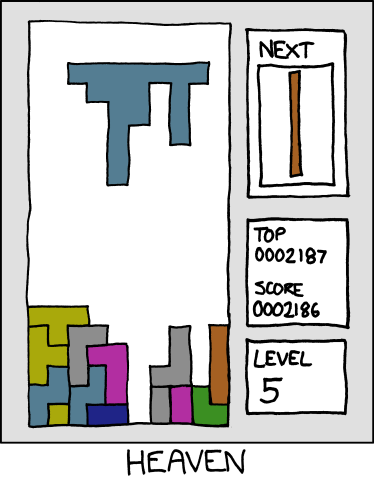
\includegraphics[scale=0.45]{xkcd/heaven}
		\end{figure}
	
		\pause
		\column{0.5\linewidth}
		\begin{figure}[H]
			\vspace{-20pt}
			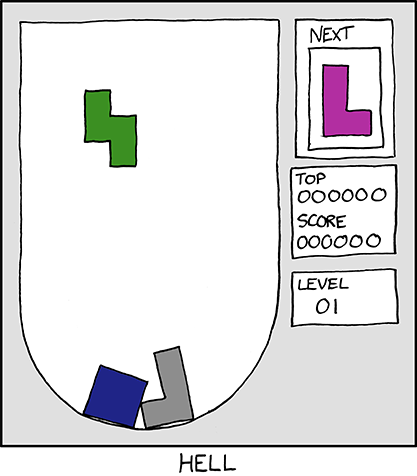
\includegraphics[scale=0.45]{xkcd/hell}
		\end{figure}
	\end{columns}
\end{frame}
}

\begin{headframe}[ Viel Erfolg  bei \\ euren Klausuren!\rlap{ \smiley}]
	--- The End ---
\end{headframe}
\mycomment{
% Scheint leider kein vernünftiges Abschieds-XKCD zu geben
\thasse{
	\xkcdframevert{287}{}{4.0}
	%\xkcdframe{5.8}{30}{xkcd/np_complete.png}{http://www.xkcd.com}{}
}
}

\slideThanks

\end{document}